\documentclass[10pt,a4paper]{article}
\usepackage[margin=21mm,headheight=15pt]{geometry}
\usepackage[T1]{fontenc}
\usepackage{lmodern,amsmath,amssymb,tikz,graphicx,hyperref,fancyhdr,enumitem}
\usetikzlibrary{arrows.meta,positioning,calc,decorations.pathmorphing}
\definecolor{ink}{RGB}{20,53,78}
\hypersetup{colorlinks=true,urlcolor=ink,linkcolor=ink}
\setlength{\parindent}{0pt}\setlength{\parskip}{5pt}
\emergencystretch=3em
\pagestyle{fancy}\fancyhf{}\fancyfoot[C]{\thepage}
\renewcommand{\headrulewidth}{.3pt}
\newcommand{\task}[2]{\par\medskip{\color{ink}\Large\bfseries #1. #2}\par\smallskip}
\newcommand{\answer}{\par\smallskip\textbf{Worked reasoning.} }
\setlist[enumerate]{label=\textbf{(\alph*)},leftmargin=7mm,itemsep=7pt}
\begin{document}
\fancyhead[L]{\small Control of Dynamical Systems}
\fancyhead[R]{\small Laboratory 02}
{\color{ink}\LARGE\bfseries Laboratory 02}\par
{\large Ventilation as a bilinear dynamical system}\par
\textbf{Worked solutions -- five integrated problems}\par
{\small\textbf{Evidence boundary.} Original hypothetical scenarios. Derive, calculate and justify decisions; every numerical record is synthetic. Figures are conceptual and not to scale.}
\smallskip\textbf{Shared nominal data.} Nominal room: $V=120$ m$^3$, source $S=360$ ppm m$^3$/min and ventilation $q_0=3$ m$^3$/min, with clean inlet air and perfect mixing. Excess concentration $c$ is in ppm. Problem 5 introduces a separate liquid analogue with explicitly different units.
\par\smallskip{\small\textbf{Study route.} On a first modeling pass, solve Problems 1--3 and 5(b). Return to Problem 4 and 5(a,c) after Laboratory 05 introduces PI feedback; revisit actuator limits after Laboratory 09.}
\task{1}{From a ventilated room to a local input--output model}
A room has a uniform excess tracer concentration. Fresh air removes tracer, and a separate source generates it. Distinguish airflow from tracer flow in the physical illustration.
\begin{center}\resizebox{\ifdim\width>.98\linewidth.98\linewidth\else\width\fi}{!}{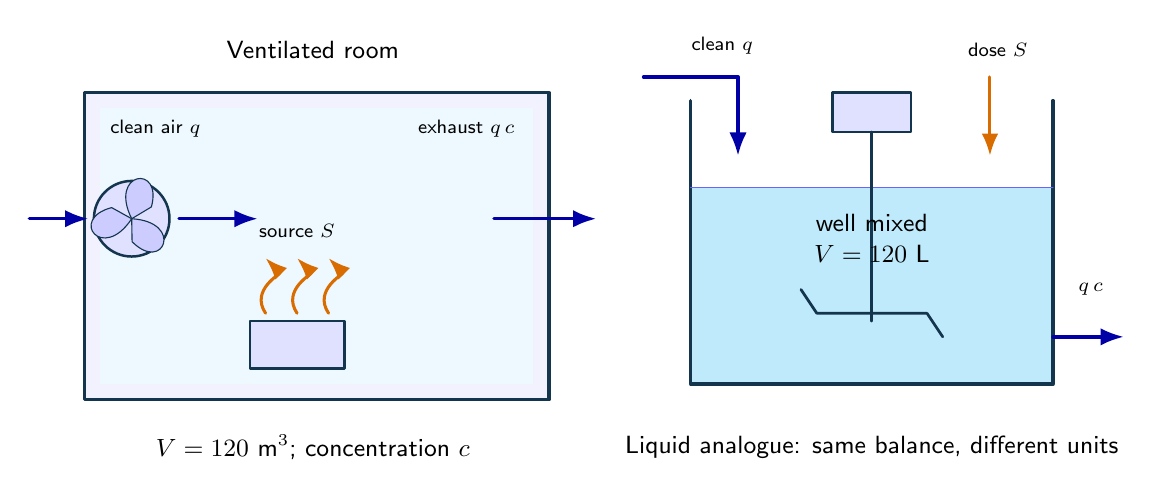
\begin{tikzpicture}[
font=\sffamily\small,>=Latex,line cap=round,line join=round,
wall/.style={draw=ink,line width=1.2pt,fill=blue!5},
water/.style={fill=cyan!25,draw=none},
metal/.style={draw=ink,fill=blue!12,line width=.9pt},
flow/.style={->,draw=blue!65!black,line width=1.2pt},
heat/.style={->,draw=orange!85!black,line width=1.1pt},
measure/.style={->,draw=teal!70!black,line width=.9pt},
dim/.style={<->,draw=ink!65,line width=.6pt},
spring/.style={draw=ink,decorate,decoration={coil,aspect=.5,segment length=4pt,amplitude=3pt}},
wire/.style={draw=ink,line width=1pt},
lab/.style={align=center,font=\sffamily\small},
smalllab/.style={align=center,font=\sffamily\scriptsize}]

\draw[wall](.3,.2)--(.3,4.1)--(6.2,4.1)--(6.2,.2)--cycle;
\fill[cyan!7](.5,.4)rectangle(6,3.9);
\draw[metal](.9,2.5)circle(.48);
\foreach \a in {0,120,240}{\draw[ink,fill=blue!20,rotate around={\a:(.9,2.5)}](.9,2.5)..controls(.6,3.1)and(1.3,3.2)..(1.15,2.65)--cycle;}
\draw[flow](-.4,2.5)--(.35,2.5);
\draw[flow](1.5,2.5)--(2.5,2.5);
\draw[flow](5.5,2.5)--(6.8,2.5);
\node[smalllab]at(1.2,3.65){clean air $q$};
\node[smalllab]at(5.15,3.65){exhaust $q\,c$};
\draw[metal](2.4,.6)rectangle(3.6,1.2);
\foreach \x in {2.6,3,3.4}{\draw[heat](\x,1.3)..controls(\x-.2,1.6)and(\x+.2,1.8)..(\x,2);}
\node[smalllab]at(3,2.35){source $S$};
\node[lab]at(3.2,4.65){Ventilated room};
\node[lab]at(3.2,-.4){$V=120$ m$^3$; concentration $c$};
\fill[water](8,.4)rectangle(12.6,2.9);
\draw[wall,fill=none](8,4)--(8,.4)--(12.6,.4)--(12.6,4);
\draw[blue!60](8,2.9)--(12.6,2.9);
\draw[flow](7.4,4.3)--(8.6,4.3)--(8.6,3.3);
\draw[flow](12.6,1)--(13.5,1);
\draw[metal](9.8,3.6)rectangle(10.8,4.1);
\draw[wire](10.3,3.6)--(10.3,1.2);
\draw[wire](9.6,1.3)--(11,1.3)(9.6,1.3)--(9.4,1.6)(11,1.3)--(11.2,1);
\draw[heat](11.8,4.3)--(11.8,3.3);
\node[smalllab]at(11.9,4.65){dose $S$};
\node[smalllab]at(8.4,4.7){clean $q$};
\node[smalllab,anchor=west]at(12.8,1.6){$q\,c$};
\node[lab]at(10.3,2.25){well mixed\\$V=120$ L};
\node[lab]at(10.3,-.4){Liquid analogue: same balance, different units};
\end{tikzpicture}
}\par{\small A ventilated room and a well-mixed liquid analogue share an inventory balance. The room uses m$^3$ and the liquid case uses L; do not mix their concentration or flow units. Equal inlet and outlet volume flows keep each inventory constant.}\end{center}
\begin{enumerate}
\item A well-mixed volume has $V=120$ m$^3$, source $S=360$ ppm m$^3$/min and ventilation $q$ in m$^3$/min. Derive the balance for excess concentration $c$ and the equilibrium and time constant at $q_0=3$.
\answer Tracer accumulation is $V\dot c=S-qc$, with all terms in ppm m$^3$/min. At constant $q_0=3$, $c_0=S/q_0=120$ ppm. The homogeneous exponent is $-q_0/V$, giving $\tau=V/q_0=40$ min. This is excess concentration relative to constant inlet concentration. The units of $S$ encode concentration times volume per time, not pure mass per time.
\item Linearize $V\dot c=S-qc$ about $(S_0,q_0,c_0)=(360,3,120)$. Retain source and ventilation deviations as inputs. Give both transfer functions and the term neglected by linearization.
\answer Write $c=c_0+\delta c$, $q=q_0+\delta q$, and $S=S_0+\delta S$. Subtracting the equilibrium gives $120\delta\dot c=\delta S-3\delta c-120\delta q-\delta q\delta c$. Dropping the product yields $\delta C/\delta S=1/(120s+3)$ and $\delta C/\delta Q=-120/(120s+3)=-40/(40s+1)$. More airflow decreases excess concentration, hence the negative sign. Validity depends on small deviations, not merely on smooth input signals.
\item For nonzero $\delta c$, compare the discarded bilinear term with the retained term $q_0\delta c$. Give a useful local smallness condition and explain why it is not a complete error bound for a long transient.
\answer Expanding gives $V\delta\dot c=\delta S-q_0\delta c-c_0\delta q-\delta q\,\delta c$. The magnitude ratio of the discarded term to $q_0\delta c$ is $|\delta q|/q_0$ when $\delta c\ne0$. Thus small relative airflow changes support the local approximation. This comparison does not bound every forcing term, accumulated trajectory error or parameter uncertainty; it is a local scale argument, not a global validity certificate.
\end{enumerate}

\newpage
\task{2}{Testing a linearization with progressively larger airflow steps}
Keep the source fixed and increase airflow from its nominal value. Compare exact equilibria, local predictions and the time needed to cross a concentration threshold.
\begin{enumerate}
\item Starting from 120 ppm, increase flow to 3.3 m$^3$/min while retaining the source. Derive the exact trajectory and the local-model prediction. Compare their equilibria and time constants.
\answer The exact equilibrium is $360/3.3=1200/11$ ppm and the exact time constant is $120/3.3=400/11$ min. Thus $c=1200/11+(120-1200/11)e^{-11t/400}$. The local prediction is $c_{lin}=120-12(1-e^{-t/40})$, with final value 108 ppm and time constant 40 min. It underestimates the exact final concentration by $12/11\approx1.091$ ppm. Linearization changes both the equilibrium shift and the rate for this finite perturbation.
\item Repeat the flow change with $q=6$. Find both equilibrium predictions and the exact time to reach 75 ppm. Explain whether the zero equilibrium predicted by the local model is physically attainable with a positive source.
\answer The exact final value is $360/6=60$ ppm and $\tau=20$ min, giving $c=60+60e^{-t/20}$. Therefore $75=60+60e^{-t/20}$ leads to $t=20\ln4\approx27.73$ min. The local model predicts $120-120(1-e^{-t/40})$ and final value zero. At finite flow and positive source, equilibrium requires $c=S/q>0$; the zero prediction is an extrapolation error, not a valid operating point.
\item Let $q=q_0(1+\varepsilon)$ with $\varepsilon>-1$. Derive exact and linearized equilibrium concentration, their absolute difference and their relative difference measured against the exact concentration. Evaluate the last quantity for $\varepsilon=0.1$ and 1.
\answer At fixed source, $c_{\rm exact}=c_0/(1+\varepsilon)$, while $c_{\rm lin}=c_0(1-\varepsilon)$. Subtraction yields $c_{\rm exact}-c_{\rm lin}=c_0\varepsilon^2/(1+\varepsilon)\ge0$. Dividing by $c_{\rm exact}$ gives the relative discrepancy $\varepsilon^2$: 1 percent for a 10 percent airflow increase and 100 percent when flow doubles. A negative local concentration beyond this range is a model failure, not a physically attainable negative tracer inventory.
\end{enumerate}

\newpage
\task{3}{A feedforward specification under source uncertainty}
The ventilation actuator has finite capacity. Design decisions must account both for the largest disturbance and for uncertainty in its magnitude.
\begin{center}\resizebox{\ifdim\width>.98\linewidth.98\linewidth\else\width\fi}{!}{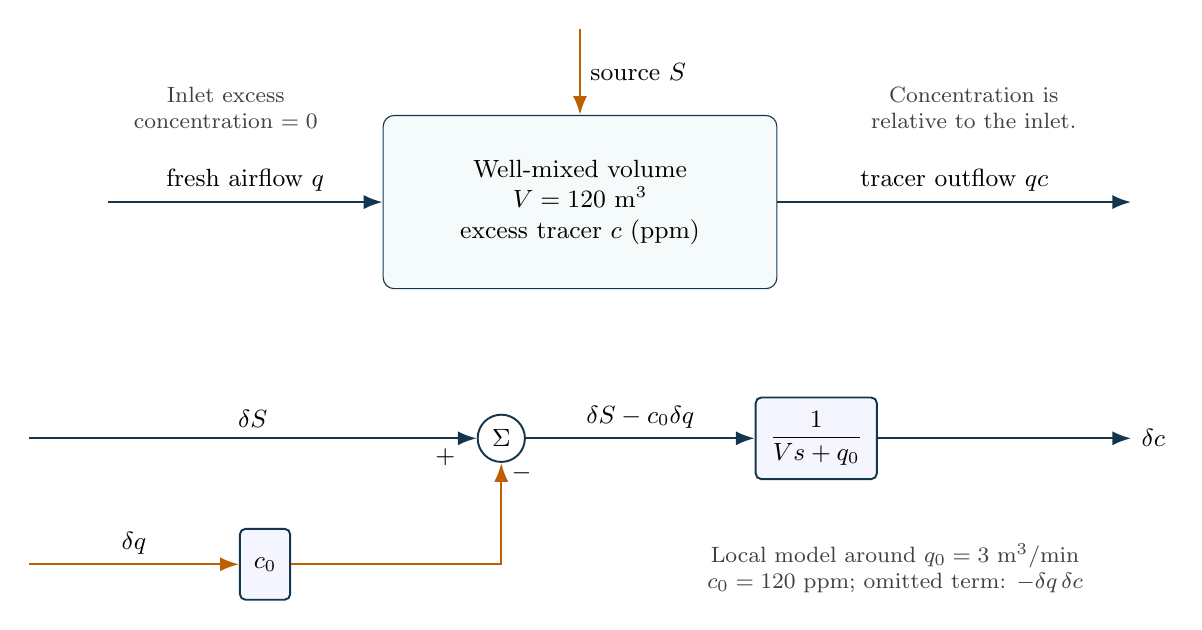
\begin{tikzpicture}[x=1cm,y=1cm,>=Latex,font=\small,
block/.style={draw=ink,fill=blue!4,rounded corners=2pt,minimum height=9mm,align=center,line width=.7pt,inner sep=5pt},
sum/.style={circle,draw=ink,fill=white,minimum size=6mm,inner sep=0pt,line width=.7pt},
sig/.style={->,draw=ink,line width=.85pt},
fb/.style={->,draw=teal!70!black,line width=.85pt},
dist/.style={->,draw=orange!75!black,line width=.85pt},
tap/.style={circle,fill=ink,inner sep=1.4pt},
note/.style={font=\footnotesize,align=center,text=black!75}]

\node[draw=ink,fill=teal!4,rounded corners,minimum width=50mm,minimum height=22mm,align=center](v)at(7,2.3){Well-mixed volume\\$V=120\ \mathrm{m^3}$\\excess tracer $c$ (ppm)};
\draw[sig](1,2.3)--node[above]{fresh airflow $q$}(v.west);
\draw[sig](v.east)--node[above]{tracer outflow $qc$}(14,2.3);
\draw[dist](7,4.5)--node[right]{source $S$}(v.north);
\node[note]at(2.5,3.5){Inlet excess\\concentration $=0$};
\node[note]at(12,3.5){Concentration is\\relative to the inlet.};
\node[sum](s)at(6,-.7){$\Sigma$};
\node[block](p)at(10,-.7){$\dfrac{1}{Vs+q_0}$};
\node[block](gain)at(3,-2.3){$c_0$};
\draw[sig](0,-.7)--node[above]{$\delta S$}node[pos=.93,below]{$+$}(s);
\draw[dist](0,-2.3)--node[above]{$\delta q$}(gain);
\draw[dist](gain)--(6,-2.3)--node[pos=.9,right]{$-$}(s);
\draw[sig](s)--node[above]{$\delta S-c_0\delta q$}(p);
\draw[sig](p)--(14,-.7)node[right]{$\delta c$};
\node[note]at(11,-2.35){Local model around $q_0=3\ \mathrm{m^3/min}$\\$c_0=120\ \mathrm{ppm}$; omitted term: $-\delta q\,\delta c$};

\end{tikzpicture}
}\par{\small The physical balance and its local two-input signal model. Airflow enters with a negative sign because increased ventilation removes excess tracer.}\end{center}
\begin{enumerate}
\item The target excess concentration is 100 ppm and the source rises from 360 to 480 ppm m$^3$/min. Find the required feedforward flows. If flow is limited to 4 m$^3$/min, find the final concentration after the source change.
\answer Equilibrium feedforward satisfies $q_{ff}=S/c_{target}$. The required flows are 3.6 and 4.8 m$^3$/min. The latter exceeds the actuator limit. At $q=4$ and $S=480$, the attainable equilibrium is $c=480/4=120$ ppm. No controller can maintain 100 ppm with this source and limit under the stated model. The constraint must be checked before tuning the feedback law.
\item At fixed flow $q=3.6$, the source is only known to lie in $[324,396]$. Find the equilibrium interval and the flow needed to guarantee an equilibrium no larger than 110 ppm under that source uncertainty.
\answer Because $c_\infty=S/q$ increases monotonically with $S$, the fixed-flow interval is $[324/3.6,396/3.6]=[90,110]$ ppm. To enforce $S/q\le110$ for every allowed source, use the largest source: $q\ge396/110=3.6$ m$^3$/min. This is an equilibrium statement under the mixing model, not a bound on every transient or a health recommendation.
\item Now use the uncertain source interval $[324,396]$ ppm m$^3$/min, require $c_\infty\le100$ ppm and retain maximum flow 4 m$^3$/min. Find the smallest constant flow that guarantees the requirement and the corresponding concentration interval.
\answer The worst source requires $396/q\le100$, so $q\ge3.96$ m$^3$/min. This lies below the 4 m$^3$/min limit. At the smallest feasible flow the interval is $[324/3.96,396/3.96]=[81.818\ldots,100]$ ppm. This guarantee uses the stated bounded source and steady model. It does not cover the separate 480-unit source case, for which the same 4-unit capacity gives 120 ppm.
\end{enumerate}

\newpage
\task{4}{Choosing the feedback sign and checking the resulting operating point}
The controller increases fresh airflow when excess concentration rises above its target. Use the nonlinear balance to check a controller designed from the local model.
\begin{enumerate}
\item Use $q=q_0+k(c-c_{ref})$ near $c_{ref}=c_0=120$. Derive the local closed-loop pole and choose $k$ for a 20 min time constant. Specify the units of $k$.
\answer The local equation with no source perturbation is $120\delta\dot c=-(3+120k)\delta c$. Its pole is $-(3+120k)/120$. For a 20 min time constant, $3+120k=6$, hence $k=0.025$ (m$^3$/min)/ppm. A positive concentration error increases flow, which reduces concentration. The resulting negative feedback follows from the plant's negative input gain. This calculation ignores flow saturation.
\item With the proportional law of Problem 4(a), a constant source increment of 60 ppm m$^3$/min occurs. Find the local steady concentration and flow deviations. Then find the exact positive equilibrium of the nonlinear balance and compare.
\answer The local equilibrium satisfies $0=60-6\delta c$, giving $\delta c=10$ ppm and $\delta q=0.25$ m$^3$/min. Exactly, $q=3+0.025(c-120)=0.025c$, so $420=0.025c^2$. The positive equilibrium is $c=\sqrt{16800}\approx129.6148$ ppm, with $q\approx3.24037$. The local model slightly overestimates the change. Proportional feedback leaves an offset after an unknown source change.
\item For the 60-unit source increment, calculate the exact equilibrium airflow with the specified proportional controller and check the limit $q\le4$. Explain why neither more proportional gain nor integral action can maintain 100 ppm when $S=480$ and this limit applies.
\answer At $r=120$, $q=3+0.025(c-120)=0.025c$. With $S=420$, $0.025c^2=420$, so $c=\sqrt{16800}\simeq129.6148$ ppm and $q\simeq3.24037$ m$^3$/min, within capacity. By contrast, $S=480$ and $c=100$ require $q=4.8$, outside capacity. Integral action can change the equilibrium error only when the required actuator effort is available; otherwise saturation and windup must be considered.
\end{enumerate}

\newpage
\task{5}{The same balance in a stirred dilution vessel}
Use the liquid analogue shown beside the room: an ideally mixed 120 L vessel receives clean water at $q$ L/min and a negligible-volume solute dose $S=360$ mg/min. Equal inlet and outlet flows maintain volume. Here $c_{ref}=120$ mg/L; the gains in part (a) use consistent L, mg and min units.
\begin{enumerate}
\item Let $e=c-c_{ref}$, $q=q_0+k_p e+z$, and $\dot z=k_i e$. Derive the linear characteristic polynomial. For $k_p=0.025$ and $k_i=0.0004$, calculate natural frequency and damping ratio.
\answer The deviation equations are $\dot e=-(3+120k_p)e/120-z$ and $\dot z=k_i e$. Thus the polynomial is $s^2+(0.025+k_p)s+k_i$. With the given gains it is $s^2+0.05s+0.0004$, so $\omega_n=0.02$ min$^{-1}$ and $2\zeta\omega_n=0.05$, giving $\zeta=1.25$. Its roots are $-0.01$ and $-0.04$ min$^{-1}$. Positive integral gain is consistent with the chosen error sign.
\item Assume constant $S\ge0$, $q>0$ and $c(0)\ge0$. Prove that the exact concentration stays nonnegative and tends to $S/q$. Give two reasons a local model or this mixing model can be misleading in practice.
\answer The exact solution is $c(t)=c(0)e^{-qt/V}+(S/q)(1-e^{-qt/V})$. For $t\ge0$, both coefficients are nonnegative and sum to one; the solution lies between its nonnegative initial value and equilibrium. Since the exponential vanishes, it tends to $S/q$. A local model can predict negative concentrations under large changes. The mixing model can miss spatial gradients, time-varying sources or inlet conditions. These are mathematical teaching scenarios, not exposure assessments.
\item Map the room model to this vessel, state the new concentration units, and evaluate the feasibility of a 100 mg/L target when $S=480$ mg/min and $q\le4$ L/min. Explain the consequence for the proposed integral controller.
\answer Replace room excess concentration by liquid concentration in mg/L, room volume by 120 L and airflow by water flow in L/min. The same balance $120\dot c=S-qc$ follows, now with every term in mg/min. Its nominal concentration is 120 mg/L and time constant 40 min. At $S=480$ the minimum attainable equilibrium concentration is 120 mg/L, so the 100 mg/L target is infeasible. An unconstrained integrator keeps increasing its flow request while the physical actuator remains saturated. The numerical analogy preserves coefficients, not physical units.
\end{enumerate}

\end{document}
